\begin{figure}[htbp]
\centering
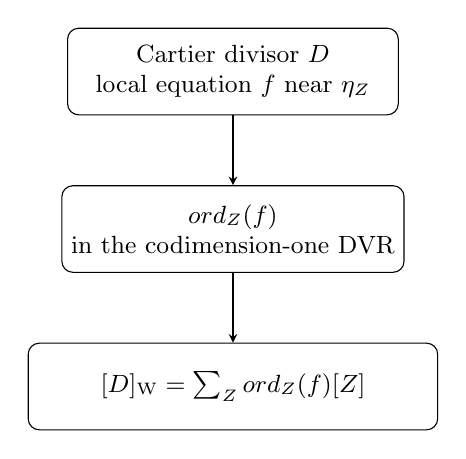
\begin{tikzpicture}[>=stealth,every node/.style={font=\small}]
\node[draw,rounded corners,minimum width=4.2cm,minimum height=1.1cm,align=center] (c) at (0,1.5) {Cartier divisor $D$\\local equation $f$ near $\eta_Z$};
\node[draw,rounded corners,minimum width=4.2cm,minimum height=1.1cm,align=center] (v) at (0,-0.5) {$\operatorname{ord}_Z(f)$\\in the codimension-one DVR};
\node[draw,rounded corners,minimum width=5.2cm,minimum height=1.1cm] (w) at (0,-2.5) {$[D]_{\mathrm W}=\sum_Z\operatorname{ord}_Z(f)[Z]$};
\draw[->] (c)--(v);
\draw[->] (v)--(w);
\end{tikzpicture}
\caption{On a normal Noetherian integral scheme, codimension-one valuations send Cartier divisors injectively to Weil divisors.}
\label{fig:vi40-cartier-weil}
\end{figure}
